\begin{frame}[fragile]
  \frametitle{Globally-Visible Objects: Chares and Proxies}
  \begin{center}
    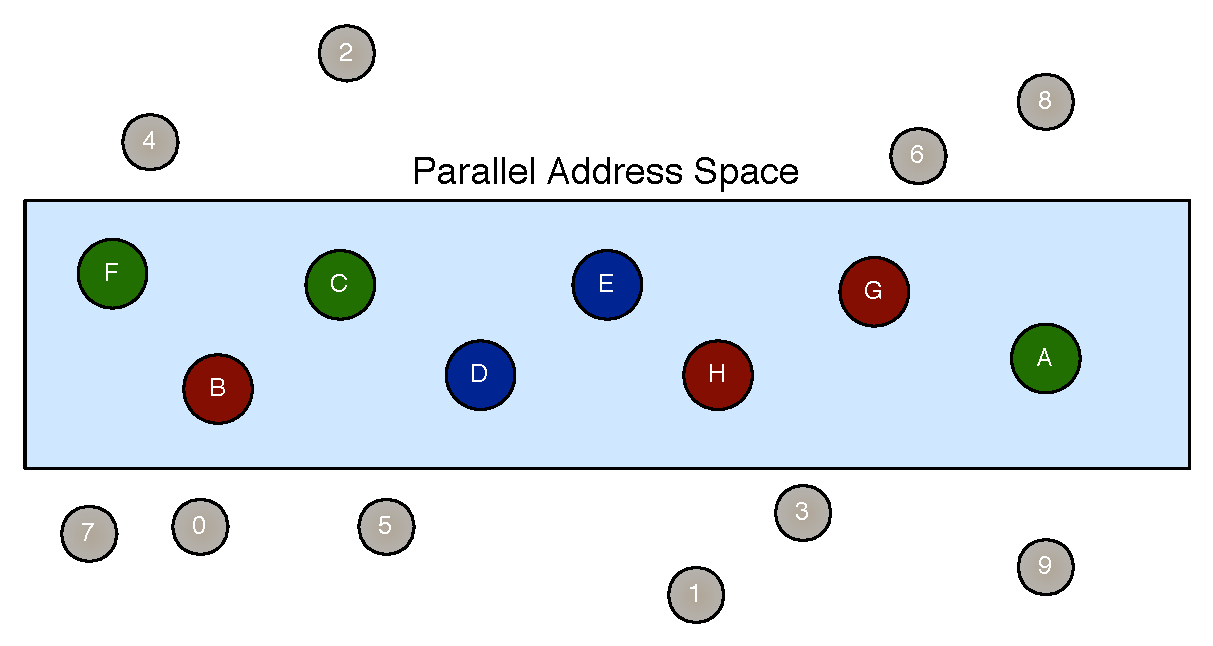
\includegraphics[width=0.8\textwidth]{figures/objectGlobalAddress.pdf}
  \end{center}
  \begin{itemize}
    \item Certain ``special'' object \emph{instances} are:
      \begin{itemize}
      \item first-class citizens in the parallel address space,
      \item with unique location-independent names
      \end{itemize}
    \item Under the hood, the runtime handles locality and provides the
      mechanisms to promote objects to the parallel space
  \end{itemize}
\end{frame}

\begin{frame}[fragile]
  \frametitle{Globally-Visible Methods: Entry Methods}
  \begin{center}
    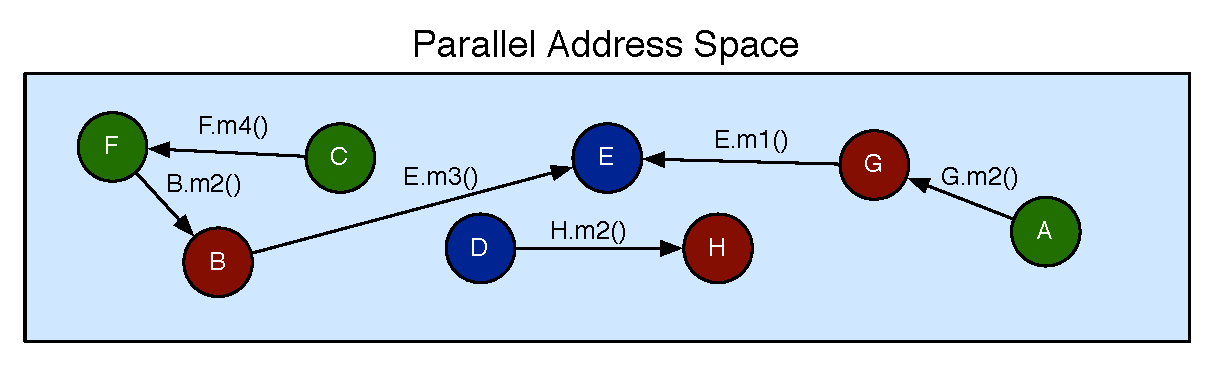
\includegraphics[width=\textwidth]{figures/objectMethodGlobalAddress.pdf}
  \end{center}
  \begin{itemize}
    \item How can objects communicate across address spaces?
      \begin{itemize}
      \item Just like a sequential object-oriented language, an object's
        reference is used to invoke a method
      \item In the parallel space, this is a handle that is location
          transparent
      \item A method invocation becomes an act of communication
      \end{itemize}
  \end{itemize}
\end{frame}

\begin{frame}[fragile]
  \frametitle{Method-Driven Asynchronous Communication}
  \begin{center}
    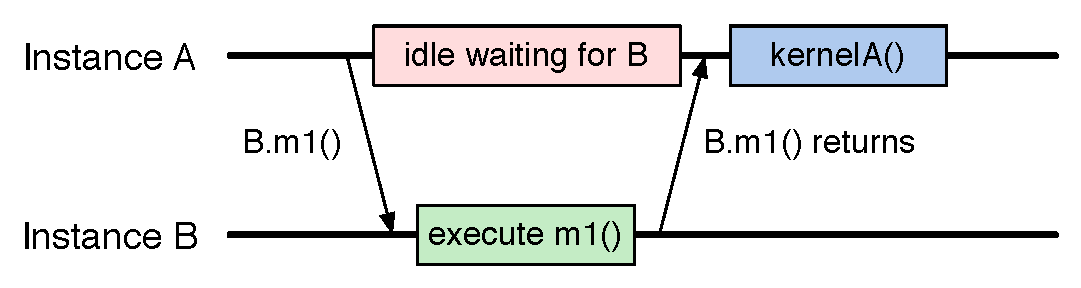
\includegraphics[width=\textwidth]{figures/objectSequence.pdf}
  \end{center}
  \begin{itemize}
  \item What happens if an object waits for a return value from a method
    invocation?
    \begin{itemize}
    \item Performance
    \item Latency
    \item Reasoning about correctness
    \end{itemize}
  \end{itemize}
\end{frame}

\begin{frame}[fragile]
  \frametitle{Design Principle: Do not wait for remote completion}
  \begin{center}
    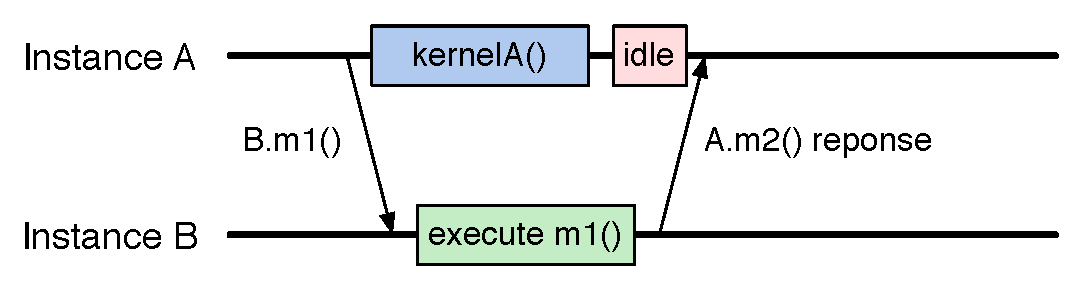
\includegraphics[width=\textwidth]{figures/objectSequenceAsync.pdf}
  \end{center}
  \begin{itemize}
  \item Hence, method invocations should be asynchronous
    \begin{itemize}
    \item No return values
    \end{itemize}
  \item Computations are driven by the incoming data
    \begin{itemize}
    \item Initiated by the sender or method caller
    \end{itemize}
  \end{itemize}
\end{frame}

\begin{frame}
  \frametitle{For example, a Jacobi reduction}
  \begin{center}
    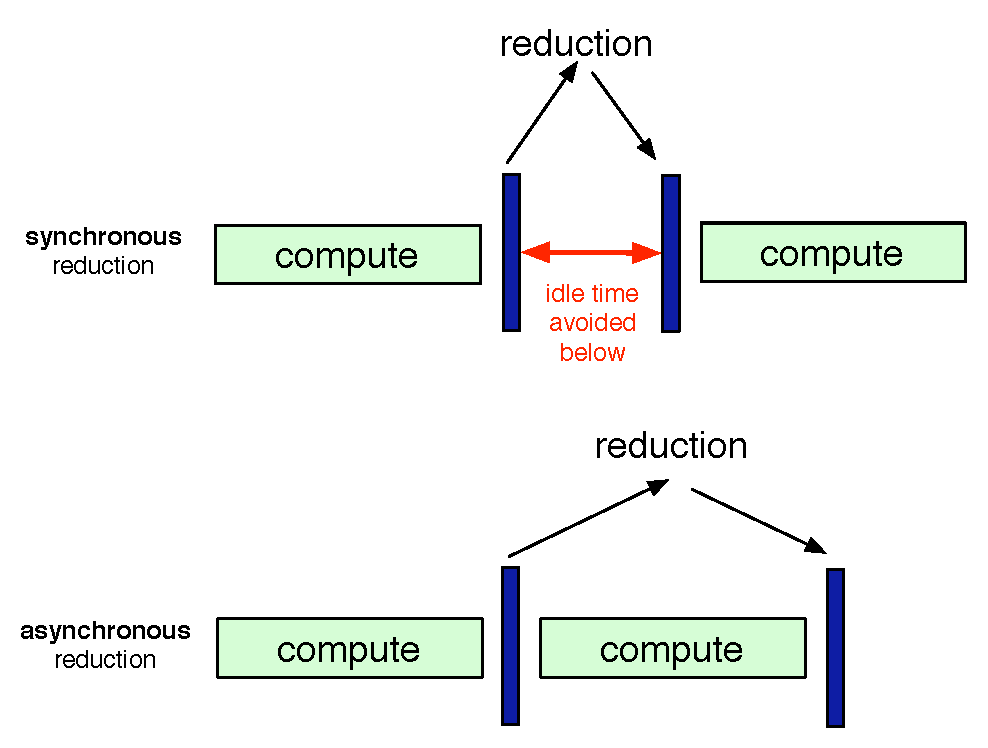
\includegraphics[width=0.8\textwidth]{figures/asyncReduction.pdf}
  \end{center}
\end{frame}

\begin{frame}[fragile]
  \frametitle{Methods: Natural Units of Sequential Computation}
  \begin{columns}
    \begin{column}{0.55\textwidth}
      \begin{itemize}
      \item Methods still have the same sequential semantics
        \begin{itemize}
        \item Atomicity: methods do not execute in parallel
        \end{itemize}
      \item Methods cannot be interrupted  or preempted
      \item Methods interact and update state of an object in the same way
      \item Method sequencing is what changes from sequential computation
      \end{itemize}
    \end{column}
    \begin{column}{0.45\textwidth}
      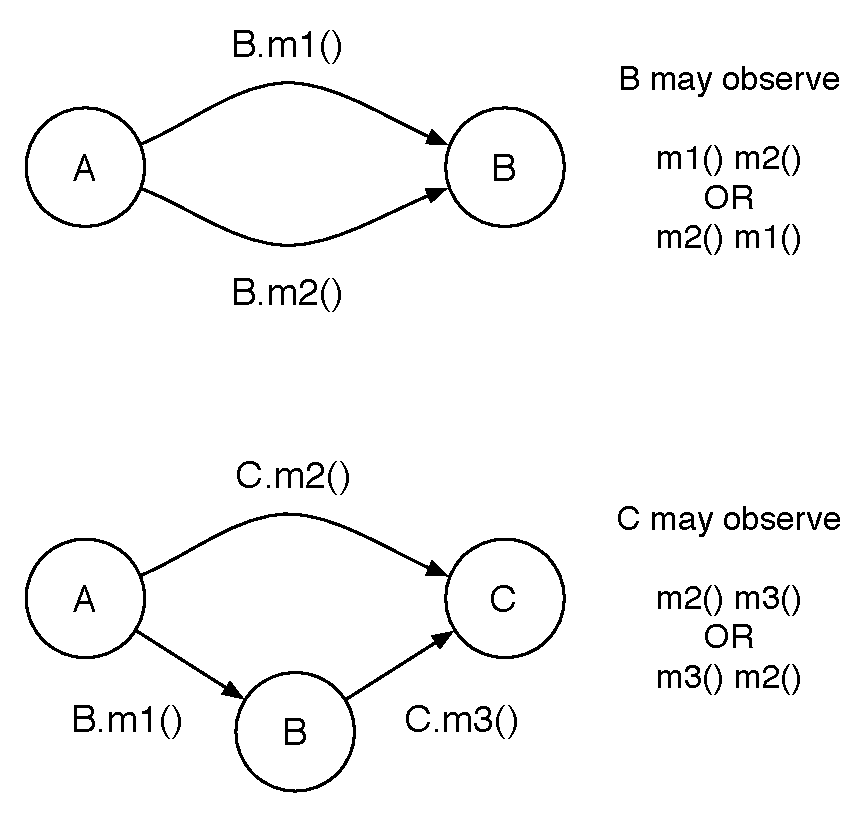
\includegraphics[width=1\textwidth]{figures/sequencing.pdf}
    \end{column}
  \end{columns}
\end{frame}

% \begin{frame}[fragile]
%   \frametitle{Dependencies and Dataflow}
%     \begin{columns}
%     \begin{column}{0.55\textwidth}
%       \begin{itemize}
%       \item A method invocation expresses a dependency in the computation
%       \item For example, we can now express a LU decomposition in its natural
%         form
%         % \begin{itemize}
%         % \item A directed acyclic graph
%         % \end{itemize}
%       \item More sophisticated dependencies can be expressed with a scripting
%         language in Charm++
%       \end{itemize}
%     \end{column}
%     \begin{column}{0.45\textwidth}
%       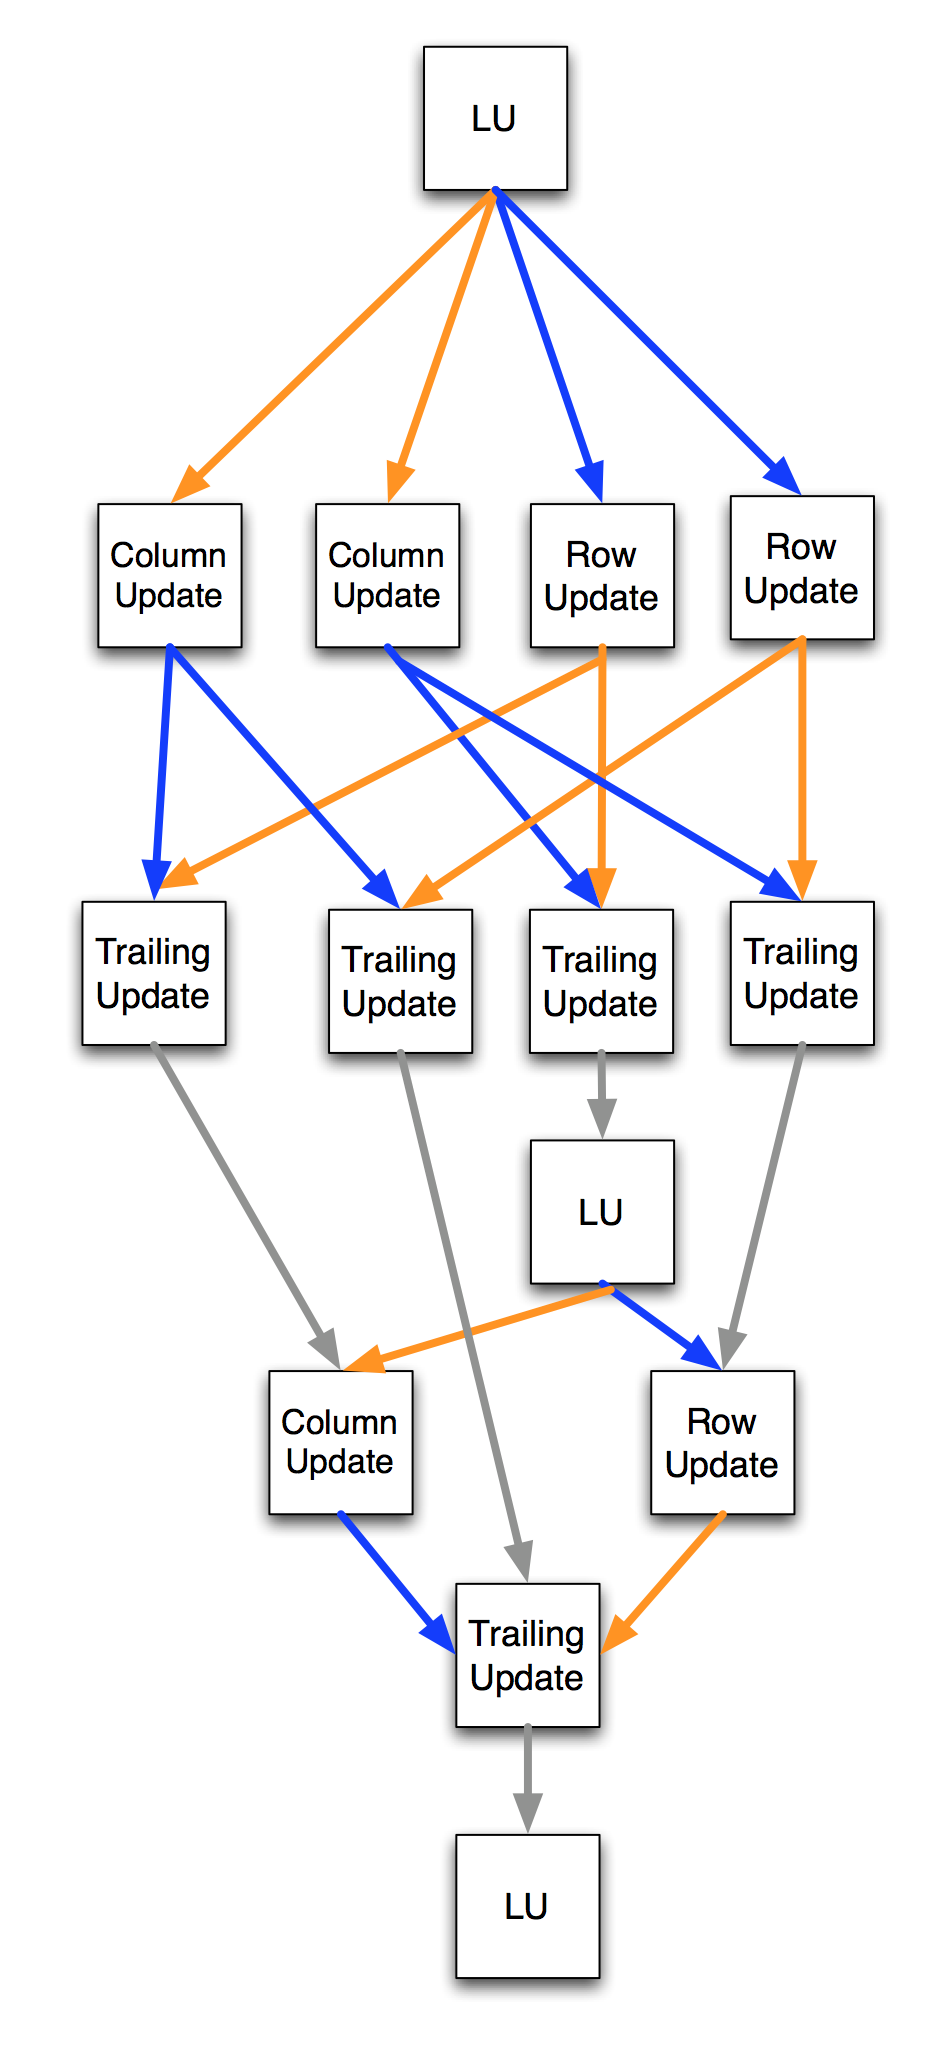
\includegraphics[width=0.7\textwidth]{figures/ludag.png}
%     \end{column}
%   \end{columns}
% \end{frame}
